\chapter{Chi tiết các service}
\label{ch:chi-tiet-cac-service}

Chương~\ref{ch:kien-truc-va-du-lieu}  đã trình bày kiến trúc tổng thể của hệ thống, 
bao gồm vai trò của các service, phạm vi dữ liệu mà mỗi service quản lý và cách chúng giao tiếp với nhau. 
Tiếp nối nội dung đó, chương này tập trung phân tích ba service đảm nhiệm các chức năng xử lý chính: 
\texttt{backend}, \texttt{agent} và \texttt{document}.

\section{Backend}
\label{sec:be}

\subsection{Vai trò và trách nhiệm}

\texttt{backend} là \textbf{gateway} (cửa vào duy nhất) của hệ thống: mọi yêu cầu từ màn hình của
giáo viên hay học sinh đều tới nó qua một lời gọi \textbf{API} (giao diện lập trình), và không màn
hình nào gọi thẳng một service khác. Với mỗi lời gọi, \texttt{backend} xác định người gọi là ai,
kiểm dữ liệu được hỏi có thuộc về người ấy không và trạng thái hiện tại có cho phép thao tác ấy
không, rồi mới đọc hay ghi \textbf{database} (cơ sở dữ liệu). Mọi dữ liệu nghiệp vụ trong database
đều do \texttt{backend} ghi, trừ kết quả và tiến độ xử lý tài liệu, do \texttt{ingest} ghi.

Phần lớn lời gọi được trả lời ngay sau một lần đọc hay ghi database. Ba loại lời gọi thì trả về qua
\textbf{SSE} (kết nối giữ mở): hội thoại của giáo viên, hội thoại của học sinh và thư viện tài liệu
(mục~\ref{sec:hang-doi}). Qua kết nối ấy, \texttt{backend} gửi từng \textbf{event} (sự kiện) xuống
màn hình mỗi khi có gì mới.

Những phần xử lý chạy lâu --- viết bằng mô hình ngôn ngữ, hay đọc một tệp vừa tải lên --- thì
\texttt{backend} không tự làm. Nó giao chúng đi dưới dạng \textbf{job} (một đầu việc, một lần chạy)
qua \textbf{queue} (hàng đợi) của \texttt{redis}, kèm \textbf{task} là tên của loại việc ấy: sáu
task của \texttt{agent} trong bảng~\ref{tab:bay-viec}, và một task dò tệp cho \texttt{document}, tức
xem tệp có sẵn chữ hay là bản chụp; task này không gọi mô hình nên không có trong bảng ấy.
\texttt{agent} không được ghi vào database, nên mọi thứ nó viết ra đều về qua \texttt{backend}, và
\texttt{backend} quyết định ghi gì. Nhưng \texttt{backend} không có \textbf{worker} (tiến trình nền)
nào: nó chỉ chạy khi có một lời gọi đi qua. Điều này quyết định cách nó lấy kết quả của các job đã
giao, trình bày ở mục kế tiếp.

\subsection{Giao job, lấy kết quả và gửi event}

\paragraph{Ba cách lấy kết quả.} Không phải job nào cũng cần kết quả ngay, nên \texttt{backend} lấy
kết quả một job của \texttt{agent} theo một trong ba cách, tuỳ việc ai cần kết quả ấy và cần lúc nào
(bảng~\ref{tab:be-lay-ket-qua}).

\begin{table}[htb]
\centering
\caption[Ba cách \texttt{backend} lấy kết quả một job của \texttt{agent}]{Ba cách \texttt{backend} lấy kết quả một job của \texttt{agent}, và giới hạn mặc định của mỗi cách}
\label{tab:be-lay-ket-qua}
\begin{tabular}{@{}L{4.0cm}L{7.0cm}L{3.6cm}@{}}
\toprule
\textbf{Cách} & \textbf{Dùng cho} & \textbf{Giới hạn mặc định} \\
\midrule
Lấy kết quả ngay trong lời gọi & Ba task của hội thoại giáo viên; câu biến thể khi phải viết tại chỗ & 70 giây cho một job \\
\addlinespace
Chuyển chữ hiện dần, rồi lấy kết quả & Trả lời một tin nhắn của học sinh & 25 giây không có chữ mới \\
\addlinespace
Giao job, thu hoạch sau & Viết một câu hỏi của đề; viết trước câu biến thể & Kết quả còn đọc được trong 1 giờ \\
\bottomrule
\end{tabular}
\end{table}

Cách thứ nhất dùng khi người dùng đang nhìn màn hình và lời gọi chỉ trả lời được khi đã có kết quả,
như một bước của lượt hội thoại, hay câu biến thể học sinh cần ngay để làm: \texttt{backend} giữ lời
gọi mở cho tới khi job xong. Cách thứ hai cũng giữ lời gọi mở, nhưng chuyển từng mảnh chữ
\texttt{agent} vừa viết xuống màn hình ngay khi nó tới, nên học sinh đọc được câu trả lời trong lúc
nó còn đang được viết. Vì vậy giới hạn của cách này đo khoảng im lặng chứ không đo độ dài: mỗi mảnh
chữ mới tới thì đồng hồ tính lại từ đầu. Cách thứ ba dùng khi không lời gọi nào cần đứng lấy kết quả
của từng job: soạn câu cho đề, mỗi câu một job chạy độc lập, và cả bộ có khi mất vài phút. Câu biến
thể cũng được viết trước theo cách này, ngay lúc học sinh nộp bài, để thời gian viết rơi vào lúc em
đang đọc giải thích và hỏi trợ lí ở giai đoạn 2. Riêng job dò tệp của \texttt{document} không thuộc
cách nào: không ai lấy kết quả của nó, vì kết quả đi về qua \texttt{ingest}
(mục~\ref{sec:noi-chuyen}).

\paragraph{Thu hoạch.} Với cách thứ ba, không lời gọi nào đứng lấy kết quả của từng job, và vì
\texttt{backend} không có worker nên cũng không có tiến trình nền nào nhận thay. Kết quả nằm trong
\texttt{redis} một giờ rồi mất. Báo cáo gọi việc \texttt{backend} lấy những kết quả đã xong ấy về,
kiểm từng cái, ghi cái đạt vào database và giao lại cái không đạt là \emph{thu hoạch}.

Thu hoạch chạy theo hai đường. Đường thứ nhất: lời gọi nào đọc hay sửa một đề đang soạn cũng thu
hoạch đề ấy trước, như xem chi tiết đề, duyệt đề, xoá câu, soạn thêm hay thay một câu; ở phía học
sinh, mở màn hình chữa bài hay mở một lượt làm lại thì thu hoạch câu biến thể viết trước. Đường thứ
hai chỉ có khi giáo viên đang xem lượt hội thoại vừa giao việc soạn câu: mỗi khi \texttt{agent} báo
một câu vừa xong, \texttt{backend} thu hoạch ngay rồi gửi số câu mới xuống màn hình.

Hệ quả là một lời gọi chỉ đọc cũng có thể ghi vào database: xem chi tiết một đề có thể đưa thêm câu
mới vào đề, còn mở màn hình chữa bài có thể giao thêm job viết trước câu biến thể. Đây là lựa chọn
có cân nhắc. Thứ được ghi là kết quả đã có sẵn, và thu hoạch hai lần không sinh thêm gì; còn nếu
không thu hoạch, giáo viên sẽ nhìn một đề trống trong khi các câu đã viết xong và đang nằm trong
\texttt{redis}.

\paragraph{Thông báo và event.} \texttt{backend} nghe ba loại \textbf{channel} (kênh) trên
\texttt{redis}, theo cơ chế \textbf{pub/sub} (phát tin lên kênh, ai đang nghe thì nhận): chữ hiện
dần của câu trả lời cho học sinh, thông báo một câu của đề đang soạn vừa xong, và thông báo thư viện
tài liệu của một giáo viên vừa đổi. Ở cả ba chỗ, \texttt{backend} bắt đầu nghe \emph{trước}, vì
pub/sub không giữ lại thứ đã phát. Với chữ hiện dần và câu soạn xong, nó nghe rồi mới giao job; với
thư viện tài liệu, nó nghe rồi mới báo màn hình đọc lại danh sách, để lần đọc ấy bù cho thông báo
nào đã phát trước lúc bắt đầu nghe.

Event gửi xuống màn hình thì khác nhau tuỳ chỗ. Event của hội thoại giáo viên mang đủ dữ liệu để màn
hình vẽ ngay, và mỗi event chỉ được gửi sau khi bước của nó đã ghi vào database, nên tải lại trang
vẫn dựng lại được đúng những gì đã hiện. Học sinh nhận từng mảnh chữ, rồi một event kết thúc hoặc
một event báo lỗi. Thư viện tài liệu chỉ nhận một event báo có gì vừa đổi, rồi tự gọi lại danh sách.
Số câu đã soạn hiện trên màn hình cũng luôn được đếm lại từ database, không cộng dồn từ thông báo,
vì một thông báo có thể mất và một vị trí thử lại có thể báo hai lần.

\subsection{Xử lý các nghiệp vụ chính}

Bốn phần dưới đây đi qua bốn nhóm nghiệp vụ \texttt{backend} phụ trách. Luồng nghiệp vụ đã có ở
chương~\ref{ch:luong-nghiep-vu}; ở đây chỉ nói \texttt{backend} kiểm gì và quyết định gì trong từng
luồng.

\begin{figure}[p]
  \centering
  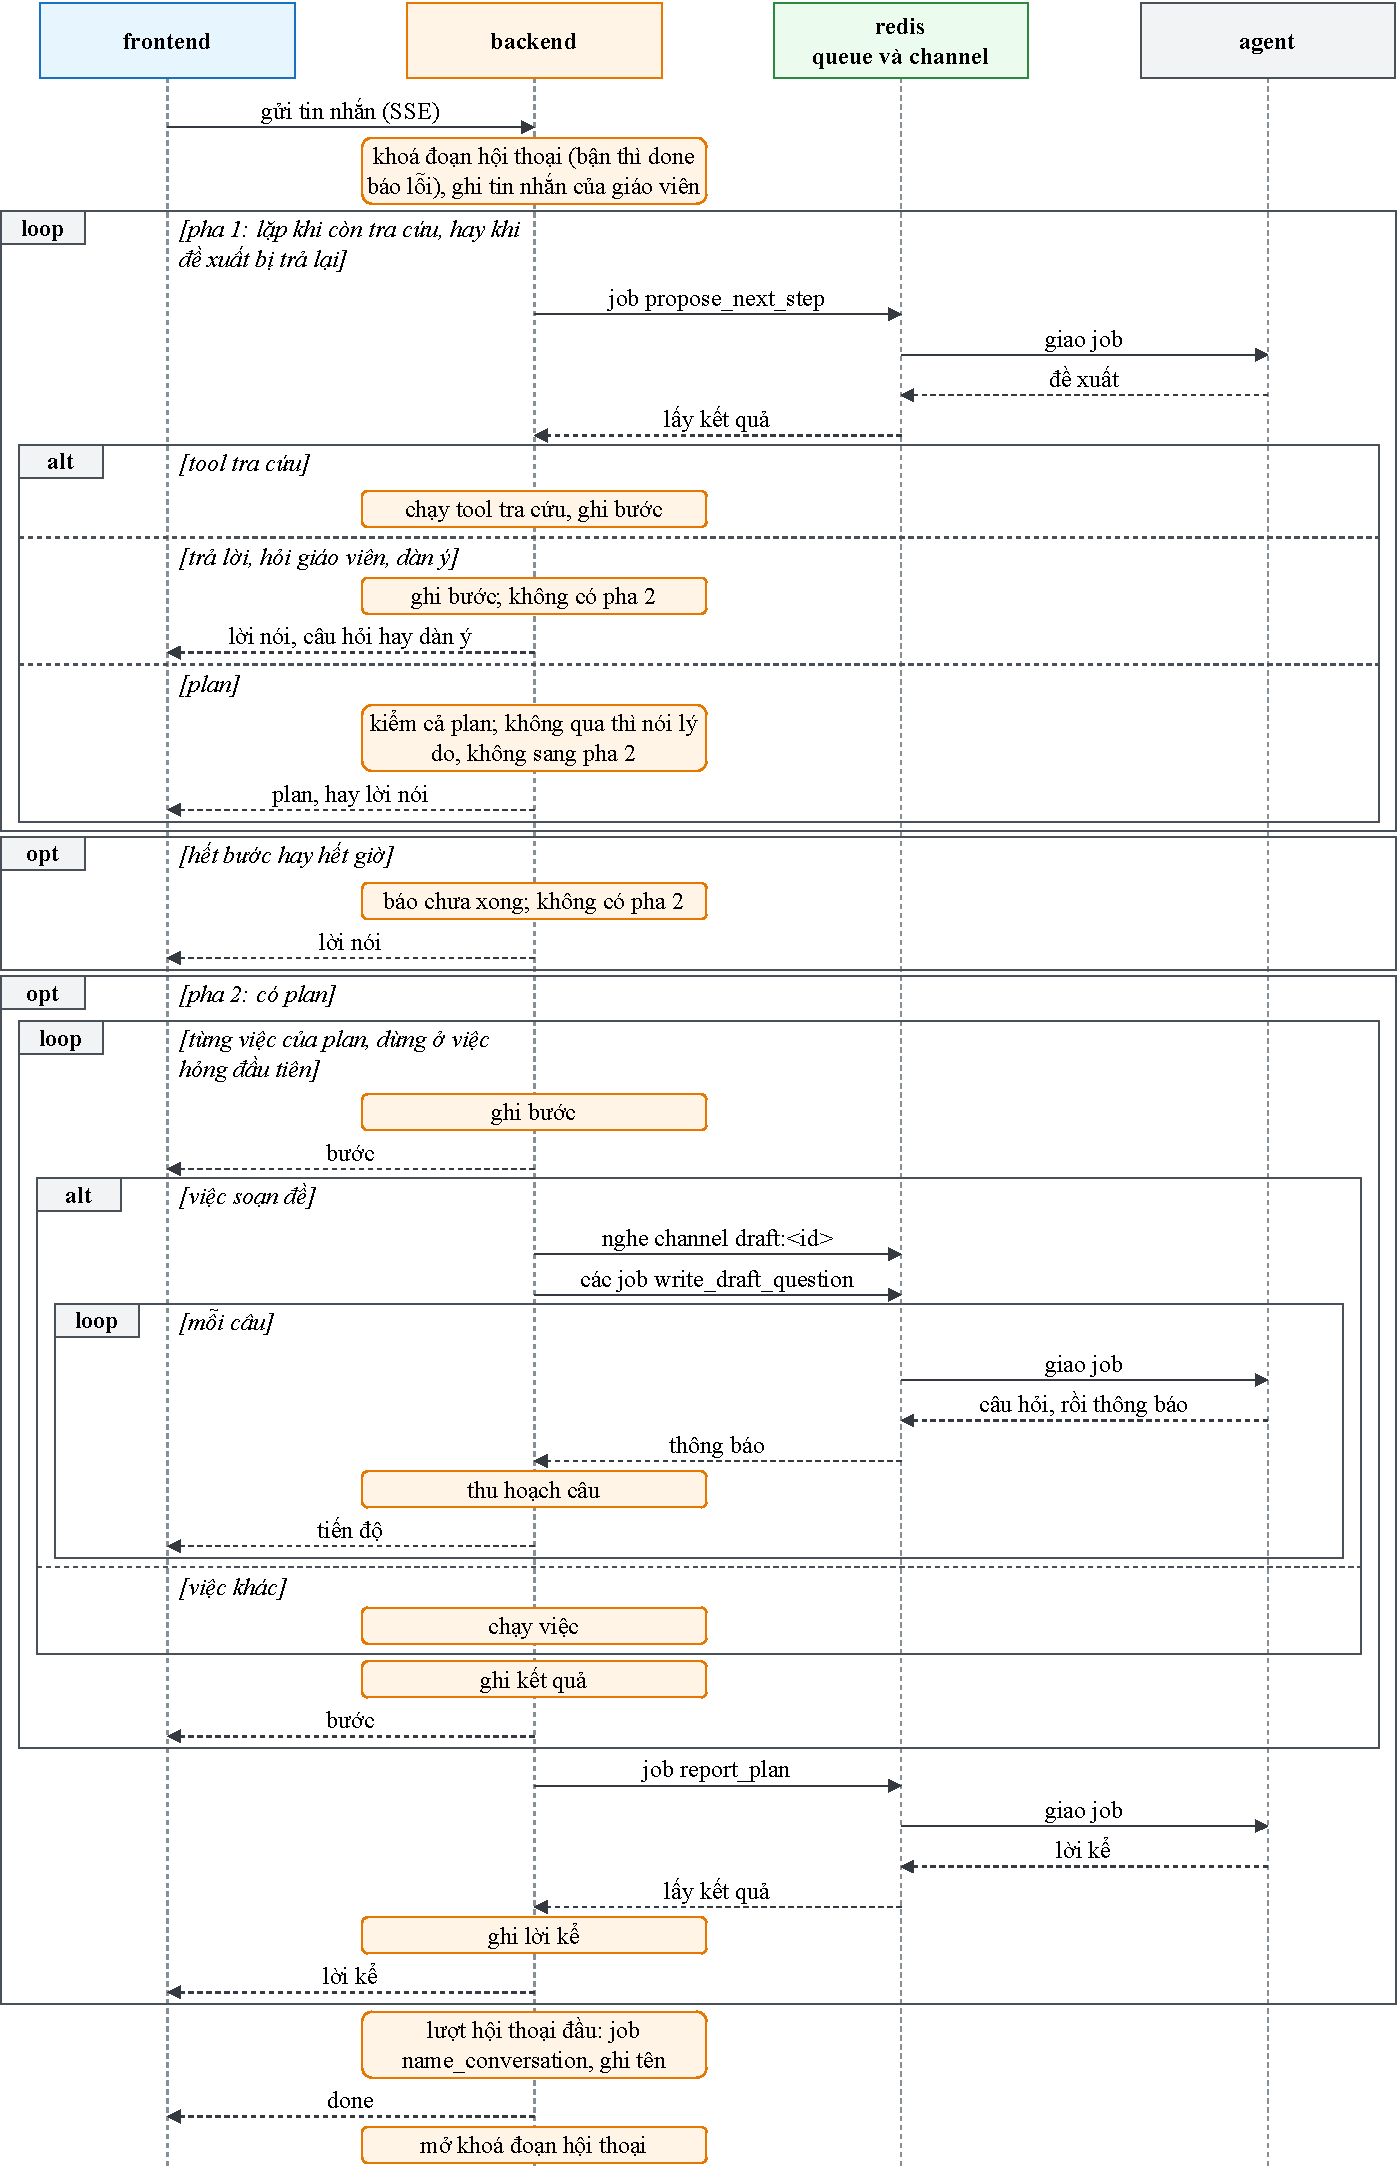
\includegraphics[width=\linewidth,height=0.95\textheight,keepaspectratio]{teacher-chat-turn.pdf}
  \caption[Một lượt hội thoại của giáo viên]{Một lượt hội thoại của giáo viên, qua SSE}
  \label{fig:teacher-chat-turn}
\end{figure}

\paragraph{Điều phối lượt hội thoại của giáo viên.} Hình~\ref{fig:teacher-chat-turn} vẽ trọn một
lượt hội thoại. Trước khi ghi gì, \texttt{backend} khoá đoạn hội thoại bằng một câu lệnh ghi có điều
kiện trên database, nên khi hai thẻ trình duyệt cùng gửi thì chỉ một thẻ được chạy; thẻ kia nhận một
event báo đoạn hội thoại đang bận. Sau đó lượt hội thoại đi qua hai pha.

Ở pha 1, mỗi bước là một job hỏi \texttt{agent} nên làm gì tiếp, và \texttt{backend} lấy kết quả
ngay trong lời gọi. \texttt{agent} có thể xin chạy một \textbf{tool} (công cụ) tra cứu, như xem lớp,
xem kết quả một đề, đọc mục lục hay chữ của tài liệu; kết quả được đưa lại cho nó ở bước sau. Pha 1
dừng khi \texttt{agent} trả lời bằng lời, hỏi lại giáo viên hay đưa ra một dàn ý --- khi đó lượt hội
thoại kết thúc --- hoặc khi nó nêu một \textbf{plan} (danh sách việc trợ lí định làm). Pha 1 có hai
trần. Trần tám bước chặn một mô hình cứ tra cứu mãi, vì mỗi bước là một lần gọi mô hình phải trả
tiền. Trần chín mươi giây cần thêm, vì tám bước mà bước nào cũng chạm giới hạn bảy mươi giây thì dài
hơn chín phút; hết chín mươi giây thì pha 1 không mở bước mới. Mỗi phần tài liệu được đọc cộng thêm
một bước và mười giây, tối đa mười phần.

Điểm cốt lõi của luồng này là \texttt{agent} chỉ đề xuất: không thao tác nào nó nêu tự chạy được. Ở
pha 1, \texttt{backend} chỉ chạy tool tra cứu; một tool ghi mà \texttt{agent} xin chạy ngay bị trả
lại kèm lời nhắc rằng tool ấy chỉ nêu được trong plan. Một dàn ý cũng được \texttt{backend} kiểm,
rồi dựng chữ từ chính các mục và lưu lại trước khi hiện ra, nên thứ giáo viên đọc đúng là thứ các
job soạn câu sẽ nhận. Khi \texttt{agent} nêu plan, \texttt{backend} kiểm plan trước khi việc nào
chạy, bằng hai phép kiểm có hậu quả khác nhau. Plan có soạn câu trước hết phải theo đúng dàn ý vừa
hiện ra cho giáo viên ở lượt hội thoại ngay trước: số câu, đề và tài liệu mà plan bỏ trống thì
\texttt{backend} điền từ dàn ý đã lưu, còn plan nêu khác dàn ý, hay chưa có dàn ý nào, thì bị trả
lại cho \texttt{agent} để sửa ngay trong lượt hội thoại, tốn thêm một bước của pha 1. Sau đó
\texttt{backend} kiểm \emph{cả} plan: không quá tám việc, vì mỗi việc là một lần ghi và một plan quá
dài có thể để lại hàng loạt đề rỗng mang tên giáo viên; mỗi việc gọi một tool ghi có thật và đủ tham
số; một việc dùng kết quả của việc khác thì chỉ được trỏ tới việc đứng trước nó. Plan trượt phép
kiểm này thì không việc nào chạy, và lượt hội thoại kết thúc bằng một câu xin giáo viên nói lại.
Không có tool nào duyệt hay phát hành đề, nên hai thao tác ấy chỉ xảy ra khi giáo viên tự bấm.

Ở pha 2, \texttt{backend} tự chạy từng việc của plan theo thứ tự, không hỏi lại \texttt{agent} nên
làm gì. Kết quả của mỗi việc được ghi vào database rồi mới gửi event, và lượt hội thoại dừng ở việc
hỏng đầu tiên. Việc soạn câu đi theo cách thứ ba trong bảng~\ref{tab:be-lay-ket-qua}, và lượt hội
thoại nghe thông báo để thu hoạch cho tới khi các câu về đủ. Cuối cùng, \texttt{backend} giao một
job riêng để \texttt{agent} kể lại kết quả, kèm số câu đếm từ database; nếu đoạn hội thoại vừa mở ở
lượt này thì thêm một job đặt tên cho nó. Khoá được mở ở cuối, kể cả khi lượt hội thoại hỏng giữa
chừng.

\paragraph{Soạn đề và vòng đời của đề.} Một lần soạn mười câu thành mười job, mỗi job một vị trí.
Mọi job của một lần soạn mang cùng một bản yêu cầu đã lưu, có số phiên bản: câu nào về mang phiên
bản cũ thì bị bỏ, và đề còn câu đang soạn thì không mở được lần soạn mới. Khi thu hoạch một câu,
\texttt{backend} cho nó qua phép kiểm câu hỏi: đúng một đáp án đúng, các phương án không trùng nhau,
mỗi phương án nhiễu gắn một lỗi, và ít nhất hai lời giải; rồi so đề bài với các câu đã có để chống
trùng. Câu đạt được đặt vào đúng vị trí giáo viên xin, không theo thứ tự nó về. Câu bị loại thì vị
trí ấy được giao lại ngay, kèm đề bài của mọi câu đã có trong đề, kể cả câu vừa ghi, để
\texttt{agent} tránh, tối đa ba lần thử. Khi thay một câu, câu cũ ở lại trong đề cho tới khi câu mới
đạt, rồi hai câu được tráo trong một lần ghi; đề đã có học sinh làm thì không thay câu được.

Duyệt chỉ đi qua khi \texttt{backend} đã thu hoạch mọi câu vừa xong, không còn câu nào đang soạn, và
đề có ít nhất một câu; trong cùng lần ghi ấy, mọi câu được chép vào ngân hàng câu hỏi. Từ lúc đó,
mọi đường ghi câu đều bị từ chối, kể cả thu hoạch, cho tới khi giáo viên bỏ duyệt. Phát hành và bỏ
duyệt xử lý nhiều lớp theo hai cách ngược nhau. Một lần phát hành dùng chung một khung giờ cho mọi
lớp được chọn nhưng xét từng lớp riêng: lớp nào không phát hành được, như phát hành lại cho một lớp
đã qua giờ mở hay đã có học sinh vào làm, thì chỉ lớp ấy trượt. Còn bỏ duyệt một đề đã phát hành là
thu hồi nó khỏi mọi lớp, mà mỗi lớp chỉ thu hồi được trước giờ mở của lớp ấy. \texttt{backend} xét
hết các lớp trước: lớp nào cũng còn trước giờ mở thì thu hồi tất cả trong một lần ghi, chỉ cần một
lớp đã qua giờ mở là không lớp nào bị thu hồi.

\paragraph{Làm bài, chấm bài và giai đoạn 2.} Giờ phải xong của một \textbf{Attempt} (lần làm bài)
do \texttt{backend} đặt lúc học sinh bắt đầu; đồng hồ trên màn hình chỉ để hiển thị, còn một lựa
chọn gửi tới sau giờ ấy bị từ chối. Hai thẻ trình duyệt cùng bấm bắt đầu thì nhận lại cùng một
Attempt. Đáp án đúng không tới màn hình học sinh trước khi em nộp: câu gửi xuống không mang dấu đáp
án nào, và lời gọi xem lời giải bị từ chối khi chưa nộp. Bài được chấm ngay trong lời gọi nộp
(mục~\ref{sec:hang-doi}); sau đó \texttt{backend} giao job viết trước câu biến thể cho những câu
sai, và queue có hỏng thì lần nộp vẫn thành công.

Ở giai đoạn 2, học sinh chỉ mở được một lượt làm lại khi còn trước hạn kết thúc giai đoạn 2 và không
có lượt nào đang mở; thời lượng của lượt bị cắt xuống hạn ấy nếu vượt. Câu biến thể được xét từng
câu: câu nào đã có câu viết sẵn thì dùng ngay, câu nào chưa có thì \texttt{backend} giao một job mới
và lấy kết quả ngay trong lời gọi mở lượt, tối đa ba lần thử. Câu biến thể nào lặp lại đề bài của
câu gốc hay của các lượt trước đều bị loại. Sau mỗi lượt, điểm của một câu chỉ có thể lên, không
xuống. Hội thoại với trợ lí ở giai đoạn này dùng cách thứ hai trong bảng~\ref{tab:be-lay-ket-qua}.

\paragraph{Quản lý tài liệu.} Thư viện tài liệu chỉ có ba lời gọi: tải một tệp lên, đọc danh sách
kèm trạng thái, và nghe thư viện thay đổi qua SSE. Khi nhận một tệp, \texttt{backend} kiểm đuôi tệp,
tệp rỗng và cỡ tệp trước khi chạm tới kho nào. Sau đó \textbf{byte} (dữ liệu gốc) của tệp được cất
vào \textbf{object store} (kho tệp) trước, rồi hàng tài liệu mới được ghi vào database; ghi hàng
hỏng thì tệp vừa cất bị xoá. Thứ tự này chọn cách hỏng rẻ hơn: một tệp sót lại mà không hàng nào trỏ
tới thì không ai thấy, và có thể dọn sau, còn một hàng trỏ vào tệp không có thì hiện lên màn hình
như một tài liệu thật. Job dò tệp chỉ được giao sau khi hàng đã ghi xong, để kết quả đọc tệp không
về tới trước khi có hàng để ghi vào.

Trạng thái hiện trên màn hình được suy ra lúc đọc: tài liệu đang xử lý mà quá ba trăm giây không báo
tiến độ thì hiện là hỏng, dù database vẫn ghi là đang xử lý. Không có lời gọi riêng nào để màn hình
đọc mục lục hay chữ của tài liệu. \texttt{backend} đọc chúng từ \textbf{content store} (kho nội
dung) khi \texttt{agent} tra cứu ở pha 1, khi dựng dàn ý và khi mở một đề theo tài liệu; tên chương,
bài chỉ lên màn hình qua hội thoại, còn chữ của tài liệu thì không được gửi xuống màn hình. Job soạn
câu không nhận chữ nào của tài liệu, chỉ nhận mục dàn ý giáo viên đã xem.

\subsection{Các ràng buộc và cơ chế kiểm soát}

Bảng~\ref{tab:be-rang-buoc} tổng hợp các ràng buộc \texttt{backend} giữ, cơ chế thực thi mỗi ràng
buộc, và cách kiểm chứng rằng nó vẫn được giữ. Cột cuối có ba loại. \emph{Kiểm thử tự động} là các
ca kiểm thử gọi đúng lời gọi hay hàm ấy rồi kiểm kết quả. \texttt{check\_contract} là một chương
trình đọc thẳng mã nguồn và cấu hình của mọi service để bắt những vi phạm mà một ca kiểm thử khó
thấy, như tệp khai báo tool gọi tới hàm đổi trạng thái của đề. \emph{Ràng buộc database} thì do
chính database từ chối dữ liệu sai.

\begin{longtable}{@{}L{7.0cm}L{4.7cm}L{2.9cm}@{}}
\caption[Ràng buộc \texttt{backend} giữ]{Ràng buộc \texttt{backend} giữ, cơ chế thực thi, và cách kiểm chứng}
\label{tab:be-rang-buoc}\\
\toprule
\textbf{Ràng buộc} & \textbf{Cơ chế thực thi} & \textbf{Kiểm chứng} \\
\midrule
\endfirsthead
\toprule
\textbf{Ràng buộc} & \textbf{Cơ chế thực thi} & \textbf{Kiểm chứng} \\
\midrule
\endhead
\midrule
\multicolumn{3}{r@{}}{\small\emph{tiếp trang sau}} \\
\endfoot
\bottomrule
\endlastfoot

\multicolumn{3}{@{}l@{}}{\textbf{Phân quyền}} \\
\addlinespace
Dữ liệu của giáo viên khác trả lời như không tồn tại & Mọi truy vấn lọc theo người gọi & kiểm thử tự động \\
\cmidrule{1-3}
Học sinh không thấy đáp án trước khi nộp & Câu gửi xuống bỏ dấu đáp án; lời giải chỉ mở sau khi nộp & kiểm thử tự động \\
\cmidrule{1-3}
Không tool nào duyệt, bỏ duyệt, phát hành hay thu hồi đề & Tệp khai báo tool không gọi tới hàm đổi trạng thái & \texttt{check\_contract} \\
\cmidrule{1-3}
Ở pha 1, chỉ tool tra cứu chạy được & Danh sách tool chia theo pha & kiểm thử tự động \\
\addlinespace

\multicolumn{3}{@{}l@{}}{\textbf{Tính hợp lệ}} \\
\addlinespace
Câu hỏi được kiểm trước khi ghi & \texttt{validate\_question}; chống trùng khi thu hoạch & kiểm thử tự động \\
\cmidrule{1-3}
Plan được kiểm trọn trước khi chạy & \texttt{vet\_plan} & kiểm thử tự động \\
\cmidrule{1-3}
Câu chỉ soạn theo dàn ý giáo viên vừa thấy & \texttt{guard\_drafting} & kiểm thử tự động \\
\cmidrule{1-3}
Job soạn câu không nhận chữ thô của tài liệu & \texttt{drafting} không đọc content store & \texttt{check\_contract} \\
\addlinespace

\multicolumn{3}{@{}l@{}}{\textbf{Tính nhất quán}} \\
\addlinespace
Đề đã duyệt từ chối mọi đường ghi câu & Một phép kiểm chung mọi đường ghi câu đi qua, kể cả thu hoạch & kiểm thử tự động \\
\cmidrule{1-3}
Chỉ duyệt đề có câu, không còn câu đang soạn; chỉ phát hành đề đã duyệt & Thu hoạch rồi mới đếm câu; phát hành từ chối đề chưa duyệt & kiểm thử tự động \\
\cmidrule{1-3}
Byte của tệp cất trước, hàng tài liệu ghi sau & Lời gọi tải lên cất tệp trước; ghi hàng hỏng thì xoá tệp & kiểm thử tự động \\
\addlinespace

\multicolumn{3}{@{}l@{}}{\textbf{Điều khiển đồng thời}} \\
\addlinespace
Mỗi đoạn hội thoại chỉ chạy một lượt hội thoại một lúc & Câu lệnh ghi có điều kiện & kiểm thử tự động \\
\cmidrule{1-3}
Mỗi học sinh một Attempt cho một đề; mỗi Attempt chỉ một lượt làm lại chưa nộp & Ràng buộc duy nhất trên \texttt{attempts}, \texttt{rounds} & ràng buộc database \\
\end{longtable}

\subsection{Xử lý lỗi}

Bảng~\ref{tab:suy-giam} nói một service ngừng thì hệ thống mất gì. Bảng~\ref{tab:be-hong} nói
\texttt{backend} làm gì khi một thao tác bên trong nó hỏng, chia theo ba nhóm: job và kết quả, kết
nối SSE, khoá đoạn hội thoại và tài liệu.

\begin{longtable}{@{}L{5.6cm}L{9.0cm}@{}}
\caption[Khi một thao tác của \texttt{backend} hỏng]{Khi một thao tác bên trong \texttt{backend} hỏng}
\label{tab:be-hong}\\
\toprule
\textbf{Khi} & \textbf{\texttt{backend} làm gì} \\
\midrule
\endfirsthead
\toprule
\textbf{Khi} & \textbf{\texttt{backend} làm gì} \\
\midrule
\endhead
\midrule
\multicolumn{2}{r@{}}{\small\emph{tiếp trang sau}} \\
\endfoot
\bottomrule
\endlastfoot

\multicolumn{2}{@{}l@{}}{\textbf{Job và kết quả}} \\
\addlinespace
Không lấy được kết quả trong lúc lời gọi còn mở & Job đề xuất ở pha 1: lượt hội thoại kết thúc bằng một event lỗi. Job kể lại: thay bằng câu \texttt{backend} tự dựng từ kết quả các việc. Job đặt tên: lấy câu đầu của giáo viên, đã cắt gọn. Câu biến thể viết tại chỗ: lời gọi mở lượt làm lại báo lỗi tạm thời \\
\cmidrule{1-2}
Kết quả đã mất khỏi \texttt{redis} trước khi được thu hoạch & Câu của đề: giao lại, tính vào ba lần thử. Câu biến thể viết trước: bỏ, rồi giao lại ngay trong lời gọi mở màn hình chữa bài ấy; nếu đang mở lượt làm lại thì viết tại chỗ \\
\cmidrule{1-2}
Câu không qua phép kiểm, hay trùng câu đã có & Như hàng trên; câu của đề dừng sau ba lần thử, lý do được lưu lại nhưng chưa hiện lên màn hình. Khi thay câu thì câu cũ ở lại \\
\cmidrule{1-2}
Job soạn câu hỏng hẳn & Vị trí ấy dừng, không giao lại; khi thay câu thì câu cũ ở lại \\
\addlinespace

\multicolumn{2}{@{}l@{}}{\textbf{Kết nối SSE}} \\
\addlinespace
Quá lâu không có chữ mới khi đang trả lời học sinh & Báo lỗi qua kết nối SSE; câu trả lời dở không được lưu \\
\cmidrule{1-2}
Lượt hội thoại hỏng hay bị từ chối sau khi kết nối SSE đã mở & Gửi một event kết thúc kèm câu báo lỗi, vì lúc ấy không còn trả được mã lỗi \\
\cmidrule{1-2}
Channel của đề đang soạn gãy, hay 180 giây không có thông báo & Thôi nghe, thu hoạch một lần cuối, rồi vẫn kể lại kết quả \\
\addlinespace

\multicolumn{2}{@{}l@{}}{\textbf{Khoá đoạn hội thoại và tài liệu}} \\
\addlinespace
Đóng thẻ trình duyệt, hay tiến trình chết giữa một lượt hội thoại & Đóng thẻ: khoá vẫn được mở. Tiến trình chết: khoá quá 10 phút thì coi như đã mở \\
\cmidrule{1-2}
Không giao được job dò tệp & Hàng tài liệu ghi ngay là hỏng, kèm lý do \\
\cmidrule{1-2}
Tài liệu không báo tiến độ quá 300 giây & Đọc ra là hỏng, mà không ghi gì \\
\end{longtable}

\subsection{Các giới hạn hiện tại}

Bốn yêu cầu dưới đây đã được đặt ra cho hệ thống, nhưng \texttt{backend} mới thực thi một phần hoặc
chưa thực thi; mỗi yêu cầu có một chỗ hở cụ thể:

\begin{itemize}
  \item \textbf{Giờ kết thúc của một lượt làm lại} (chương~\ref{ch:luong-nghiep-vu}) --- lưu từng
        lựa chọn thì có kiểm giờ, nhưng nộp cả lượt thì không, nên một lượt nộp muộn vẫn được chấm.
  \item \textbf{Câu biến thể giữ cấu trúc của câu gốc} (mục~\ref{sec:tu-dien}) --- ngoài các phép
        kiểm chung của mọi câu, chỉ có phép so đề bài với câu gốc và với các lượt trước; không gì so
        cấu trúc.
  \item \textbf{Plan đã chạy thì chạy hết và được kể lại} --- giáo viên đóng thẻ trình duyệt giữa
        pha 2 thì lượt hội thoại dừng ngay ở việc đang chạy, các việc còn lại không chạy, và không
        có lời kể nào. Muốn sửa, pha 2 phải chạy thành một job trên queue, mà muốn vậy thì cần một
        worker --- thứ \texttt{backend} không có.
  \item \textbf{Giáo viên xem được báo cáo ``giải thích chưa rõ'' của học sinh}
        (chương~\ref{ch:luong-nghiep-vu}) --- \texttt{backend} mới có đường ghi báo cáo, chưa có lời
        gọi nào để giáo viên đọc chúng.
\end{itemize}

\section{Agent}

\subsection{Vai trò và trách nhiệm}

\texttt{agent} là service viết những nội dung cần tới mô hình ngôn ngữ: câu hỏi của đề, câu biến
thể, câu trả lời cho học sinh ở giai đoạn 2, đề xuất bước tiếp theo trong hội thoại của giáo viên,
lời kể lại kết quả một plan, và tên một đoạn hội thoại. Để viết, nó gọi \textbf{Model Provider} (nhà
cung cấp mô hình). Ngoài Model Provider, nó chỉ gọi thêm một thứ nằm ngoài hệ thống: Jev, mô hình
phân loại của TypeSafe AI. Mỗi lần gọi mô hình đều gửi kèm một \emph{lời dặn}, tức đoạn chữ hướng
dẫn mô hình phải viết gì; trong hội thoại của giáo viên, Jev chọn phần nào của lời dặn được nạp.

\texttt{agent} không nhận lời gọi nào từ bên ngoài và không có quyền vào database. Nó là một worker
ngồi nghe queue của mình: \texttt{backend} giao job, \texttt{agent} viết, rồi đặt kết quả vào
\texttt{redis} để \texttt{backend} lấy về. Vì không tra được database, mỗi job phải tự mang mọi thứ
nó cần: job trả lời học sinh mang theo mọi câu em làm sai, kèm các phương án, lời giải, đáp án đúng
và phương án em đã chọn, chứ không mang một mã câu hỏi rồi tự đi tra.

Thứ \texttt{agent} trả về chỉ là nội dung, không bao giờ là một quyết định: không điểm, không độ tin
cậy, không kết luận học sinh đã hiểu hay chưa. Nó cũng không tự chạy gì: một tool hay một plan nó đề
xuất chỉ chạy khi \texttt{backend} chạy nó. Dùng nội dung ấy thế nào, ghi hay bỏ, là việc của
\texttt{backend}. Ngoài giá trị trả về, \texttt{agent} còn phát hai thứ qua pub/sub: từng mảnh chữ
của câu trả lời cho học sinh, và thông báo mỗi khi viết xong một câu cho đề đang soạn.

\subsection{Nhận job, gọi mô hình và trả kết quả}

\texttt{agent} nhận job của sáu task. Mọi lần nó gọi mô hình để viết chữ đều nằm trong một
\textbf{graph} (chuỗi hàm cố định) dựng bằng thư viện LangGraph; hai task soạn câu dùng chung một
graph. Bảng~\ref{tab:agent-vao-ra} cho biết mỗi task chạy graph nào, gọi mô hình mấy lần và trả về
gì; còn khi nào mỗi task được giao thì bảng~\ref{tab:bay-viec} đã nói.

\begin{table}[htb]
\centering
\caption[Sáu task của \texttt{agent}]{Sáu task của \texttt{agent}: graph, số lần gọi mô hình, và thứ trả về}
\label{tab:agent-vao-ra}
\begin{tabular}{@{}L{4.9cm}L{2.0cm}L{3.6cm}L{3.6cm}@{}}
\toprule
\textbf{Task} & \textbf{Graph} & \textbf{Gọi mô hình} & \textbf{Trả về} \\
\midrule
\texttt{write\_draft\_question} & \texttt{authoring} & Một tới ba lần & Một câu hỏi \\
\addlinespace
\texttt{generate\_retry\_question} & \texttt{authoring} & Một tới ba lần & Một câu biến thể \\
\addlinespace
\texttt{explain\_turn} & \texttt{explain} & Một lần, trả chữ dần & Câu trả lời cho học sinh \\
\addlinespace
\texttt{propose\_next\_step} & \texttt{propose} & Một hay hai lần, sau khi Jev chọn tệp lời dặn & Một đề xuất: trả lời, hỏi giáo viên, dàn ý, tool, hay plan \\
\addlinespace
\texttt{report\_plan} & \texttt{reporting} & Một lần & Lời kể lại \\
\addlinespace
\texttt{name\_conversation} & \texttt{naming} & Một lần & Tên đoạn hội thoại \\
\bottomrule
\end{tabular}
\end{table}

\paragraph{Graph và hàm.} Mỗi hàm của graph làm một phần của job rồi trao kết quả cho hàm sau. Graph
trả lời học sinh có hai hàm: hàm đầu dựng lời dặn từ những câu em làm sai, hàm sau gửi lời dặn ấy
cho mô hình và nhận chữ về. Graph đề xuất bước tiếp theo cũng có hai hàm: dựng lời dặn, rồi gọi mô
hình chọn một đề xuất. Graph soạn câu có hai hàm, viết rồi tự kiểm, nhưng có thêm một đường vòng:
hàm tự kiểm thấy câu chưa đạt thì gửi lý do về cho hàm viết để viết một câu khác, và hàm viết chạy
tối đa ba lần. Graph kể lại và graph đặt tên chỉ có một hàm. Hàm nhận job, nói ở đoạn dưới, không
thuộc graph nào: đó là hàm worker gọi khi lấy một job xuống, và chính nó chạy graph.

\paragraph{Ba lối ra của một job.} Mỗi task có một hàm nhận job, và cả sáu hàm đi cùng một đường. Mô
hình bị tắt trong cấu hình thì hàm trả \emph{nội dung dọn trước}, tức nội dung mã nguồn tự dựng mà
không cần mô hình: một câu viết sẵn, hay vài chữ ghép từ chính job, như sáu chữ đầu của tin nhắn làm
tên đoạn hội thoại; mô hình bật thì hàm chạy graph; graph hỏng thì hàm quay về nội dung dọn trước.
Thà có một câu dọn trước còn hơn một tính năng từ chối chạy, nhưng lựa chọn ấy có cái giá, nói ở
mục~\ref{sec:agent-gioi-han}. Riêng hàm trả lời học sinh: đã phát được vài chữ rồi mới hỏng thì nó
trả về đúng những chữ đã phát làm câu trả lời, không thay bằng câu dọn trước, vì học sinh đã thấy
chúng trên màn hình.

\paragraph{Đăng ký task và thông báo.} Sáu task được đăng ký dưới đúng tên khai trong gói dùng chung
\texttt{contracts}, không dưới tên hàm, nên đổi tên một hàm không làm gãy lời giao job của
\texttt{backend}. Thông báo một câu soạn xong chỉ được phát ngay sau khi kết quả đã ghi vào
\texttt{redis}: hàm nhận job chỉ đặt sẵn thông báo; worker ghi kết quả vào \texttt{redis} khi hàm
trả về, rồi mới phát thông báo. Phát sớm hơn thì \texttt{backend} nhận thông báo, đi thu hoạch, và
chỉ gặp một kết quả chưa có. Thông báo chỉ mang số thứ tự của câu, không mang câu: pub/sub không giữ
lại gì, nên thông báo lạc thì câu vẫn nằm trong kết quả của job và \texttt{backend} vẫn thu hoạch
được. Phát hỏng thì bỏ qua, và job vẫn được tính là xong.

\paragraph{Nối mô hình.} Chỉ một tệp, \texttt{llm.py}, biết đang gọi Model Provider nào, nên đổi
Model Provider chỉ là sửa cấu hình; Jev thì đi qua một tệp riêng. \texttt{llm.py} đặt trần thời gian
mặc định hai mươi giây cho mỗi lần gửi tới Model Provider, và xếp một mô hình dự phòng sau mô hình
chính nếu cấu hình có. Hai graph soạn câu và đề xuất bước tiếp theo bắt mô hình trả lời theo một
khuôn JSON cố định, tức một bộ ô có tên sẵn mà mô hình phải điền, như đề bài, các phương án, lời
giải; ba graph còn lại nhận chữ thường. Chữ trong khuôn --- câu hỏi soạn ra, lời nói của một đề
xuất, tên các việc của plan, dàn ý --- còn đi qua một bộ dựng lại ký hiệu toán. Mô hình viết toán
bằng LaTeX, mà trong một chuỗi JSON, dấu gạch chéo đứng trước f, n, r, t hay b là mã của một ký tự
điều khiển, nên \texttt{\textbackslash frac} về tới nơi thành một ký tự điều khiển cộng với ``rac''.
Lỗi này đã lọt vào database thật ngày 05/10/2026. Bộ dựng lại đi theo một danh sách lệnh LaTeX đã
biết, nên một lệnh không có trong danh sách thì để nguyên, chứ không bị đoán sai.

\subsection{Xử lý các task chính}

Bốn phần dưới đây đi qua bốn nhóm task. Mỗi phần nói \texttt{agent} nhận gì, viết gì, và thứ nó viết
được kiểm ở đâu, nếu có; \texttt{backend} làm gì với kết quả thì mục~\ref{sec:be} đã nói.

\paragraph{Soạn câu hỏi và câu biến thể.} Hai task này dùng chung graph soạn câu, chỉ khác lời dặn.
Job soạn một câu của đề mang mục dàn ý sinh ra câu ấy: kiến thức cần kiểm, công thức và cách làm,
đúng như giáo viên đã đọc. Các job của một lần soạn chạy song song và không thấy nhau, nên mỗi job
còn được biết mình là câu thứ mấy và kiến thức của các câu khác để khỏi hỏi sang, và mang đề bài của
những câu đã có trong đề để phép tự kiểm loại một câu lặp lại; nếu vẫn trùng thì \texttt{backend}
bắt khi thu hoạch. Job câu biến thể mang câu gốc, phương án học sinh đã chọn và lỗi em mắc, cùng đề
bài của các lượt trước; đề bài câu gốc và các lượt ấy đều bị cấm lặp. Lời dặn đòi một câu cùng dạng
và cùng cách làm nhưng khác số liệu, có một phương án nhiễu ứng với đúng lỗi ấy. Viết xong, câu qua
hàm tự kiểm, xét bốn điều: đúng một đáp án đúng, mọi phương án nhiễu gắn một lỗi, ít nhất hai lời
giải, và đề bài không trùng một đề bài bị cấm. Câu không đạt thì lý do được gửi về cho hàm viết để
viết một câu khác; sau ba lần vẫn không đạt thì hàm nhận job trả nội dung dọn trước. Phép tự kiểm
này không thay phép kiểm của \texttt{backend}, vốn rộng hơn; nó chỉ để một câu sai hình dạng không
phải đi tới \texttt{backend} rồi bị giao lại.

\paragraph{Trả lời học sinh.} Mỗi tin nhắn của học sinh là một job và một lần gọi mô hình. Lời dặn
yêu cầu trợ lí giải thích chứ không kết luận --- không cho điểm, không nói em đã hiểu --- và dùng
đúng nhãn lỗi đã gắn sẵn cho phương án em chọn từ lúc soạn đề thay vì tự chẩn đoán lại, để hai học
sinh mắc cùng một lỗi được giải thích theo cùng lỗi ấy. Trong lúc mô hình viết, hàm nhận job phát
từng mảnh chữ lên channel mà \texttt{backend} đang nghe; khi job xong, cả câu trả lời vẫn được trả
về, và đó mới là thứ được lưu.

\paragraph{Đề xuất bước tiếp theo.} Đây là task phức tạp nhất: graph đề xuất chiếm hơn một phần ba
mã nguồn và ít nhất một nửa số ca kiểm thử của \texttt{agent}. Mỗi bước của pha 1 trong
hình~\ref{fig:teacher-chat-turn} là một job của task này, và đề xuất của nó đi qua ba tầng, mỗi tầng
bắt một loại sai khác.

Tầng một là chính mô hình, đề xuất trong một khuôn. Lời dặn của task này không viết liền một khối:
phần chỉ một loại việc cần nằm trong ba \emph{tệp lời dặn}, một cho việc tra lớp và kết quả, một cho
việc soạn đề, và một tệp chung. Trước khi graph chạy, Jev đọc bốn tin nhắn gần nhất và trả lời có
hay không cho từng tệp chuyên biệt; không tệp nào được chọn thì nạp tệp chung, còn Jev không trả lời
được thì nạp cả ba. Lời dặn gửi mô hình ghép từ một lõi chung, các tệp vừa chọn, tên giáo viên, tài
liệu đang đính kèm, và hai danh sách tool: tool gọi được ngay, và tool chỉ nêu được trong plan.
Những luật mà lượt hội thoại nào cũng cần nằm trong lõi, vì Jev chọn sai thì một tệp vắng mặt. Mô
hình trả về đúng một trong năm loại đề xuất: trả lời, hỏi giáo viên, đưa ra dàn ý, gọi một tool, hay
nêu plan. Khuôn chỉ có những ô có tên sẵn, nên một đề xuất sai hình dạng không qua được tầng này.

Khuôn chỉ hỏi những gì mô hình trả lời được, vì mỗi ô là một câu hỏi đặt cho nó, và không ô nào được
để ngỏ. Bài học ấy có giá: khuôn đầu tiên là nguyên kiểu dữ liệu \texttt{agent} trả cho
\texttt{backend}, nên hỏi cả những thứ mô hình không thể biết, như mã của job, và có một ô tham số
nhận bất cứ thứ gì. Model Provider từ chối thẳng mọi lần gọi vì ô ấy, và nội dung dọn trước che kín
chuyện đó sau một câu trả lời nghe hợp lý.

Tầng hai là tám luật trong \texttt{agent}, sửa đề xuất ngay sau khi mô hình trả lời. Sáu luật giữ
thứ tự tra cứu, phần lớn quanh tài liệu: plan mở đầu bằng một tool tra cứu thì tool ấy được gọi
trước, chưa đọc mục lục thì chưa được nêu plan soạn theo tài liệu, chưa đọc chữ của phần ấy thì chưa
được đưa ra dàn ý. Một đề xuất đến sớm như vậy thành một lời gọi tool tra cứu, với tham số lấy từ
chính đề xuất hay từ những gì đã có trong hội thoại, không đoán thêm; ở bước sau, mô hình nêu lại
với kết quả trong tay. Luật thứ bảy sửa lời một câu hỏi lại đứng ngay sau danh sách tài liệu, cho
khớp các nút giáo viên sẽ bấm. Luật thứ tám sửa mục đích của một dàn ý: giáo viên nói rõ là thay câu
thứ ba mà dàn ý lại viết cho cả một đề mới thì dàn ý được thu về đúng mục chứa câu ấy. Riêng khi
giáo viên vừa được xem dàn ý và trả lời bằng một câu chỉ gồm lời đồng ý, như ``ok'' hay ``được'',
thì \texttt{agent} dựng plan thẳng từ dàn ý và bỏ đề xuất của mô hình, vì sau một chữ ``ok'' mô hình
hay quên phạm vi vừa bàn.

Sau các luật sửa là các phép kiểm: plan thiếu tham số bắt buộc, đúng luật \texttt{backend} dùng khi
kiểm plan, hay có ký tự điều khiển trong tham số; dàn ý rỗng, hay có tổng số câu khác số câu mô hình
vừa ghi nhận; câu hỏi lại giáo viên có quá ít lựa chọn; hay một đề xuất không có chữ nào. Đề xuất
vấp một phép kiểm thì \texttt{agent} chạy lại graph thêm đúng một lần. Lần hai vẫn vấp thì nó giữ
lại một trong hai đề xuất để \texttt{backend} xét, chứ không tự bịa tham số hay lựa chọn; hai lần
đều rỗng thì nó trả một câu trung tính nhờ giáo viên nói lại.

Tầng ba là \texttt{backend}: đề xuất về tới đó vẫn chỉ là đề xuất, và đoạn \emph{Điều phối lượt hội
thoại của giáo viên} ở mục~\ref{sec:be} đã kể nó được kiểm những gì.

\paragraph{Kể lại và đặt tên.} Lời kể lại kết quả một plan là một job riêng, không phải một vòng nữa
của task đề xuất: nó đọc kết quả của các việc đã chạy và không cầm danh sách tool nào, nên không thể
đề xuất thêm việc. Số câu đã soạn được đưa vào như một dòng dữ liệu, dựng từ con số \texttt{backend}
đếm trong database; lời dặn cấm nói quá điều đã làm (chỗ hở của luật này ở
mục~\ref{sec:agent-gioi-han}). Đặt tên cho một đoạn hội thoại là task nhỏ nhất: một hàm, nhận câu mở
đầu của giáo viên và trả về một cái tên ngắn. Ở đây \texttt{backend} có phép kiểm thật: cái tên phải
có ít nhất một từ chung với câu mở đầu, không thì \texttt{backend} dùng chính câu mở đầu, đã làm
gọn.

\subsection{Các ràng buộc và cơ chế kiểm soát}

Bảng~\ref{tab:agent-rang-buoc} tổng hợp các ràng buộc \texttt{agent} giữ, cơ chế thực thi mỗi ràng
buộc, và cách kiểm chứng. Cột cuối dùng hai trong ba loại đã giải thích trước
bảng~\ref{tab:be-rang-buoc}; không có ràng buộc database, vì \texttt{agent} không có database.

\begin{longtable}{@{}L{7.0cm}L{4.7cm}L{2.9cm}@{}}
\caption[Ràng buộc \texttt{agent} giữ]{Ràng buộc \texttt{agent} giữ, cơ chế thực thi, và cách kiểm chứng}
\label{tab:agent-rang-buoc}\\
\toprule
\textbf{Ràng buộc} & \textbf{Cơ chế thực thi} & \textbf{Kiểm chứng} \\
\midrule
\endfirsthead
\toprule
\textbf{Ràng buộc} & \textbf{Cơ chế thực thi} & \textbf{Kiểm chứng} \\
\midrule
\endhead
\midrule
\multicolumn{3}{r@{}}{\small\emph{tiếp trang sau}} \\
\endfoot
\bottomrule
\endlastfoot

\multicolumn{3}{@{}l@{}}{\textbf{Phân quyền}} \\
\addlinespace
Kết quả chỉ mang nội dung, không mang quyết định nào, kể cả trong các trường lồng nhau & Kiểu dữ liệu trả về của mọi task chỉ có nội dung & kiểm thử tự động \\
\cmidrule{1-3}
Không có quyền vào database & Mã nguồn không nhắc tới thư viện hay thông tin kết nối database nào & \texttt{check\_contract} \\
\cmidrule{1-3}
Lời kể lại không cầm tool nào & Yêu cầu của job kể lại không có trường nào mang tool & \texttt{check\_contract} \\
\addlinespace

\multicolumn{3}{@{}l@{}}{\textbf{Tính hợp lệ}} \\
\addlinespace
Câu hỏi đúng hình dạng & Phép tự kiểm trong graph soạn câu; \texttt{backend} kiểm lại khi thu hoạch & kiểm thử tự động \\
\cmidrule{1-3}
Chữ trong khuôn đi qua bộ dựng lại ký hiệu toán & \texttt{latex\_escapes}, ở graph soạn câu và graph đề xuất & \texttt{check\_contract} \\
\addlinespace

\multicolumn{3}{@{}l@{}}{\textbf{Tính nhất quán}} \\
\addlinespace
Task đăng ký dưới đúng tên trong \texttt{contracts} & Danh sách task của worker & kiểm thử tự động \\
\cmidrule{1-3}
Thông báo câu soạn xong phát sau khi kết quả đã ghi, chỉ mang số thứ tự & Worker phát thông báo khi job đã kết thúc & kiểm thử tự động \\
\cmidrule{1-3}
Câu trả lời bị cắt giữa chừng giữ đúng những chữ đã phát & Hàm nhận job của task trả lời học sinh & kiểm thử tự động \\
\addlinespace

\multicolumn{3}{@{}l@{}}{\textbf{Thời gian}} \\
\addlinespace
Một job, kể cả lời chọn của Jev và các lần graph gọi lại mô hình, kết thúc trước khi \texttt{backend} thôi lấy kết quả & So cấu hình hai service: Jev 3 giây + 20 giây $\times$ 3 lần gọi = 63 giây, dưới 70 giây & \texttt{check\_contract} \\
\end{longtable}

Hai ràng buộc trong bảng được kiểm chứng hẹp hơn lời của chúng. Ca kiểm thử ``không mang quyết
định'' chạy mọi task hai lần, với mô hình tắt rồi bật, nhưng mô hình giả dùng khi kiểm thử không
dựng được đầu ra theo khuôn: ở lần chạy bật, ba trong sáu task vẫn rơi về nội dung dọn trước, nên
đầu ra thật của graph soạn câu và graph đề xuất chưa bị soi. Còn phép kiểm thời gian coi hai mươi
giây là trần của cả một lần gọi, trong khi đó chỉ là trần của một lần gửi: thư viện của OpenAI tự
gửi lại tới hai lần khi quá giờ, rồi mới tới mô hình dự phòng. Một lần gọi vì thế có thể dài hơn sáu
mươi giây, và \texttt{backend} có thể thôi lấy kết quả trong lúc worker vẫn đang viết.

\subsection{Xử lý lỗi}

Bảng~\ref{tab:agent-hong} nói \texttt{agent} làm gì khi mô hình hay Jev hỏng, hay khi thứ mô hình
viết vấp phép kiểm, theo từng nhóm task. Đường lùi chung là nội dung dọn trước, như đoạn \emph{Ba
lối ra của một job} đã nói; bảng cho thấy nó trông thế nào ở từng task.

\begin{longtable}{@{}L{5.6cm}L{9.0cm}@{}}
\caption[Khi một thao tác của \texttt{agent} hỏng]{Khi một thao tác bên trong \texttt{agent} hỏng}
\label{tab:agent-hong}\\
\toprule
\textbf{Khi} & \textbf{\texttt{agent} làm gì} \\
\midrule
\endfirsthead
\toprule
\textbf{Khi} & \textbf{\texttt{agent} làm gì} \\
\midrule
\endhead
\midrule
\multicolumn{2}{r@{}}{\small\emph{tiếp trang sau}} \\
\endfoot
\bottomrule
\endlastfoot

\multicolumn{2}{@{}l@{}}{\textbf{Mọi task}} \\
\addlinespace
Mô hình quá giờ hay báo lỗi & Gọi mô hình dự phòng nếu cấu hình có; vẫn hỏng thì xử lý theo từng task dưới đây \\
\addlinespace

\multicolumn{2}{@{}l@{}}{\textbf{Soạn câu hỏi và câu biến thể}} \\
\addlinespace
Câu vấp phép tự kiểm & Gửi lý do về để viết lại; hàm viết chạy tối đa ba lần, vẫn vấp thì xử lý như mô hình hỏng \\
\cmidrule{1-2}
Mô hình hỏng khi soạn một câu của đề & Trả một câu dọn trước, lấy từ sáu câu Toán cố định \\
\cmidrule{1-2}
Mô hình hỏng khi viết câu biến thể & Câu gốc thuộc bộ câu dọn trước và còn biến thể chưa dùng thì trả biến thể ấy; không thì trả lại chính câu gốc, thêm đuôi ``(đề thay số cho lượt \ldots)'' \\
\cmidrule{1-2}
Phát thông báo câu soạn xong hỏng & Bỏ qua; job vẫn xong, và \texttt{backend} vẫn thu hoạch được câu \\
\addlinespace

\multicolumn{2}{@{}l@{}}{\textbf{Trả lời học sinh}} \\
\addlinespace
Mô hình hỏng trước khi phát chữ nào & Trả một câu trả lời dọn trước \\
\cmidrule{1-2}
Mô hình hỏng giữa chừng & Trả đúng những chữ đã phát làm câu trả lời \\
\addlinespace

\multicolumn{2}{@{}l@{}}{\textbf{Đề xuất bước tiếp theo}} \\
\addlinespace
Jev chưa được cấu hình, báo lỗi, quá 3 giây, hay trả lời một hình dạng lạ & Nạp cả ba tệp lời dặn \\
\cmidrule{1-2}
Đề xuất vấp phép kiểm & Chạy lại graph đúng một lần và giữ đề xuất lần hai, trừ ba trường hợp: lần đầu có đề xuất mà lần hai rỗng hay mô hình hỏng thì giữ lần đầu; cả hai là câu hỏi quá ít lựa chọn thì giữ lần nhiều lựa chọn hơn; cả hai đều rỗng thì trả một câu trung tính nhờ giáo viên nói lại \\
\cmidrule{1-2}
Mô hình hỏng & Trả một đề xuất dọn trước, đoán việc theo vài chữ trong tin nhắn \\
\addlinespace

\multicolumn{2}{@{}l@{}}{\textbf{Kể lại và đặt tên}} \\
\addlinespace
Mô hình hỏng khi kể lại & Ghép một câu từ kết quả các việc \\
\cmidrule{1-2}
Mô hình hỏng khi đặt tên & Lấy sáu chữ đầu của câu mở đầu \\
\end{longtable}

\subsection{Các giới hạn hiện tại}
\label{sec:agent-gioi-han}

Năm yêu cầu dưới đây đã được đặt ra cho hệ thống, nhưng \texttt{agent} mới thực thi một phần hoặc
chưa thực thi. Ba yêu cầu đầu hở vì cùng một lý do: nội dung dọn trước không mang dấu nào để
\texttt{backend} nhận ra nó. Mỗi yêu cầu có một chỗ hở cụ thể:

\begin{itemize}
  \item \textbf{Câu hỏi theo đúng môn và phạm vi giáo viên xin} --- mô hình hỏng khi soạn một câu
        thì câu dọn trước là một trong sáu câu Toán cố định, bất kể môn hay phạm vi. Câu ấy đúng
        hình dạng nên qua phép kiểm của \texttt{backend}; chỉ lúc giáo viên duyệt đề mới chặn được
        nó.
  \item \textbf{Câu biến thể khác câu gốc} --- khi mô hình bật, câu gốc do mô hình viết nên không
        thuộc bộ câu dọn trước, và mô hình hỏng thì học sinh nhận lại đúng câu gốc kèm một đuôi nói
        số đã đổi. Phép so đề bài của \texttt{backend} coi đuôi ấy là một đề bài khác, nên không
        cổng nào chặn.
  \item \textbf{Đề xuất đúng việc giáo viên nhờ} --- mô hình hỏng thì đề xuất dọn trước đoán việc
        theo vài chữ trong tin nhắn, và có thể đoán sai: ``ra đề Toán lớp 10 về mệnh đề'' thành câu
        hỏi ``Bạn muốn xem lớp nào?''. Phép đoán không còn tự nêu plan soạn đề: nó chỉ nêu plan khi
        giáo viên vừa đồng ý một dàn ý. Nhưng nó vẫn đưa ra được một dàn ý tự dựng, và
        \texttt{backend} không biết một đề xuất đến từ mô hình hay từ phép đoán.
  \item \textbf{Lời kể lại không nói quá điều đã làm} --- chỉ lời dặn canh điều này. Con số trên màn
        hình do \texttt{backend} tự đếm nên không sai theo, nhưng câu mô hình viết đi thẳng lên màn
        hình mà không ai so lại.
  \item \textbf{Giáo viên đồng ý dàn ý trước khi câu được soạn} --- luật trong \texttt{agent} chỉ
        bắt câu chỉ gồm lời đồng ý; câu khác thì đề xuất của mô hình đi nguyên, và mô hình có thể
        đọc ``ok nhưng đổi câu 2'' thành đồng ý rồi nêu plan soạn câu. \texttt{backend} chỉ chứng
        minh được dàn ý đã hiện ra cho giáo viên, nên plan ấy vẫn đi qua.
\end{itemize}

\section{\texttt{document}}

\texttt{document} đọc những tệp giáo viên tải lên và dựng cây mục lục cho chúng. Khi một job của nó
bắt đầu, byte của tệp đã nằm trong object store và job đã nằm trên queue (mục~\ref{sec:noi-chuyen});
mục này kể từ lúc worker lấy job xuống tới lúc kết quả rời service.

\subsection{Vào và ra}

\texttt{document} nhận job của ba task: \texttt{probe\_document} từ \texttt{backend}, cùng hai task
nó tự giao cho chính mình, \texttt{ocr\_pages} cho lô \textbf{OCR} (đọc chữ từ ảnh) kế tiếp và
\texttt{index\_document} cho việc dựng cây. Nó gửi về queue của \texttt{ingest} job của hai task:
\texttt{document\_probed} mang kết quả, \texttt{document\_progress} báo tiến độ. Job tới mang khoá
của tệp trong object store chứ không mang byte của nó. Mọi thứ \texttt{document} ghi đều nằm ở
content store, chia thành sáu \textbf{collection} (nhóm bản ghi cùng loại,
như một bảng) mà bảng~\ref{tab:doc-kho} liệt kê.

\begin{table}[htb]
\centering
\caption[Sáu collection của content store]{Sáu collection của content store: giữ gì, ai ghi, ai đọc}
\label{tab:doc-kho}
\begin{tabular}{@{}L{2.6cm}L{5.4cm}L{3.1cm}L{3.0cm}@{}}
\toprule
\textbf{Collection} & \textbf{Giữ gì} & \textbf{Ai ghi} & \textbf{Ai đọc} \\
\midrule
\texttt{documents} & Đầu mục của bản thô, khác bảng cùng tên của database: đọc thẳng chữ có sẵn hay qua OCR, đã đọc xong chưa & đường đọc tệp & đường dựng cây \\
\addlinespace
\texttt{pages} & Chữ của từng trang, chia theo khối & đường đọc tệp & đường dựng cây \\
\addlinespace
\texttt{indexes} & Đầu mục của cây, ghi sau cùng & đường dựng cây & \texttt{backend} \\
\addlinespace
\texttt{nodes} & Các nút của cây mục lục & đường dựng cây & \texttt{backend} \\
\addlinespace
\texttt{chunks} & Các chunk của mỗi nút & đường dựng cây & \texttt{backend} \\
\addlinespace
\texttt{block\_labels} & Quyết định cho từng ứng viên tiêu đề: ai quyết, Jev đã phân vân giữa những gì; để gỡ lỗi và đo & đường dựng cây & không ai, lúc chạy \\
\bottomrule
\end{tabular}
\end{table}

\subsection{Vì sao có hai worker}

Đọc tệp và dựng cây bị giới hạn bởi hai thứ khác nhau. Worker đọc tệp chạy một job một lúc: OCR chiếm
trọn bộ xử lí, nên hai lô chạy song song chỉ tranh nhau rồi cùng chậm. Nó nạp ba mô hình OCR
một lần lúc khởi động, vì nạp lại ở mỗi lô là trả lại chừng ấy thời gian cho từng lô của một cuốn.
Worker dựng cây không nạp mô hình nào và chạy tới bốn job song song, vì phần lớn thời gian của nó là
đợi Model Provider trả lời.

Cái giá của một job một lúc là nhiều bản chụp tải lên cùng lúc được đọc xen kẽ từng lô. Từ chừng
bảy cuốn trở lên, hay bốn cuốn nếu trang dày chữ, một cuốn im quá ba trăm giây giữa hai lần báo tiến
độ, và \texttt{backend} đọc mọi cuốn đang đọc ra là hỏng.

\subsection{Một tệp đi qua service}

Hình~\ref{fig:document-pipeline} vẽ đường đi của một tệp qua hai worker.

\begin{figure}[htbp]
  \centering
  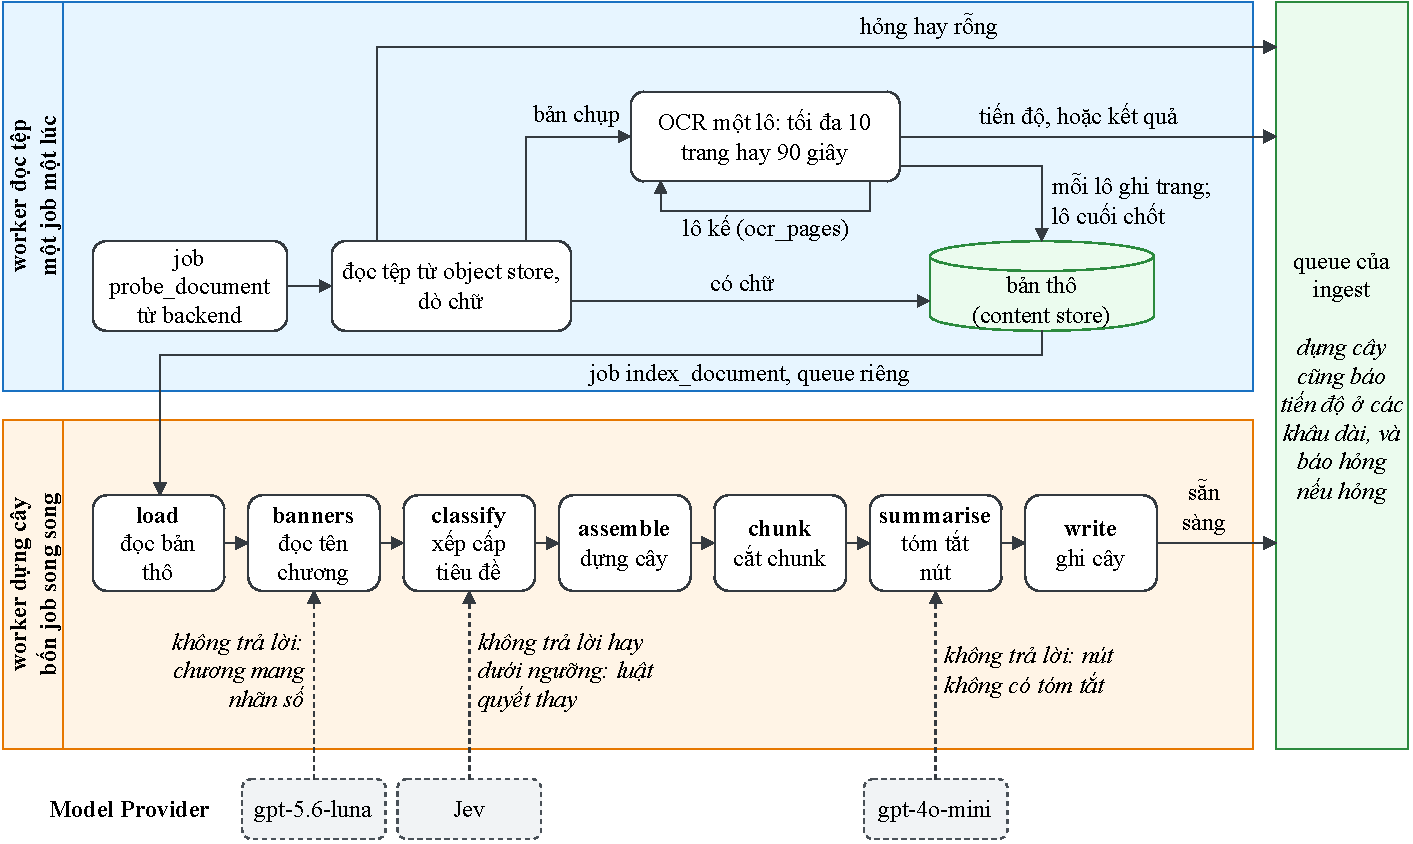
\includegraphics[width=\linewidth,height=0.5\textheight,keepaspectratio]{document-pipeline.pdf}
  \caption[Một tệp đi qua \texttt{document}]{Một tệp đi qua \texttt{document}: hai worker, ba mô hình ngoài, và các đường lùi}
  \label{fig:document-pipeline}
\end{figure}

\paragraph{Dò tệp.} Worker đọc tệp lấy byte của tệp từ object store rồi dò xem nó có chữ không. Tệp
\texttt{.txt} và \texttt{.md} phải là UTF-8, hay UTF-16 có dấu BOM; bảng mã khác bị từ chối chứ
không đoán, vì đoán sai thì ra chữ trông như chữ mà sai dấu. Với tệp PDF, nó đếm số trang có chữ, và
một trang tính là có chữ khi có từ một trăm ký tự trở lên: từ mười phần trăm số trang có chữ trở lên
thì tệp có sẵn chữ, còn lại là bản chụp. Một PDF không có trang nào bị trả về là không có chữ, không
đi OCR. Đếm trang chứ không cộng ký tự là có chủ ý: một bản chụp có một trang mục lục dày chữ vẫn
không lọt cổng.

\paragraph{Bản chụp đọc theo lô.} Một bản chụp được đọc qua nhiều job, mỗi job một lô: tối đa mười
trang, và không mở trang mới sau chín mươi giây. Mỗi lô ghi trang của nó vào content store; trừ lô
cuối, nó báo tiến độ về \texttt{ingest} rồi tự giao lô kế lên chính queue của worker đọc tệp. Mỗi
trang đi qua năm chặng: dựng ảnh, nhận khối, tìm dòng, đọc chữ từng dòng, rồi gán dòng vào khối. Hai
chặng nhận khối và tìm dòng dùng mô hình của PaddleOCR, còn chặng đọc chữ dùng EasyOCR, vì bộ đọc
chữ của PaddleOCR không bao giờ phát ra chữ tiếng Việt mang hai dấu như ``ế'' hay ``ộ''. Công thức
toán không được đọc riêng, vì lần đo trên máy chỉ có bộ xử lí trung tâm cho thấy mô hình đọc công
thức không cứu được: khối công thức chỉ nhận chữ OCR như mọi khối khác.

\paragraph{Bản thô ghi trước.} Đọc xong, \texttt{document} có một \emph{bản thô}
(mục~\ref{sec:tu-dien}) trong content store, nhưng tài liệu \emph{chưa} sẵn sàng: nó còn cần cây
mục lục. Worker đọc tệp giao một job \texttt{index\_document} lên queue riêng của worker dựng cây, và
chưa gửi kết quả nào về \texttt{ingest}.

\paragraph{Bảy khâu dựng cây.} Job dựng cây chạy một graph gồm bảy khâu nối thẳng
(bảng~\ref{tab:doc-khau}). Ba khâu gọi một mô hình ngoài, và cả ba đều có đường lùi ngay bên trong
khâu: mô hình không trả lời thì tài liệu vẫn sẵn sàng, chỉ kém hơn.

\begin{table}[H]
\centering
\caption[Bảy khâu dựng cây mục lục]{Bảy khâu dựng cây mục lục, và đường lùi của những khâu gọi mô hình}
\label{tab:doc-khau}
\begin{tabular}{@{}L{2.3cm}L{7.3cm}L{5.0cm}@{}}
\toprule
\textbf{Khâu} & \textbf{Làm gì} & \textbf{Mô hình không trả lời thì} \\
\midrule
\texttt{load} & Đọc bản thô; bản thô chưa đọc xong thì không chạy & --- \\
\addlinespace
\texttt{banners} & Đọc tên chương trên ảnh đầu chương, bằng \texttt{gpt-5.6-luna} & Chương mang nhãn số \\
\addlinespace
\texttt{classify} & Xếp vai trò và cấp cho từng tiêu đề; luật và Jev cùng quyết, Jev thắng khi đủ chắc & Luật quyết thay \\
\addlinespace
\texttt{assemble} & Dựng cây tối đa ba cấp, không nhảy cấp; tiêu đề sâu hơn gộp vào nút cha & --- \\
\addlinespace
\texttt{chunk} & Cắt chữ thành các chunk dưới từng nút & --- \\
\addlinespace
\texttt{summarise} & Tóm tắt từng nút, từ dưới lên, bằng \texttt{gpt-4o-mini} & Nút không có tóm tắt \\
\addlinespace
\texttt{write} & Ghi cây vào content store & --- \\
\bottomrule
\end{tabular}
\end{table}

Mô hình không dựng cây. Ở khâu \texttt{classify}, luật và Jev cùng đưa ra một quyết định cho mỗi
tiêu đề, và Jev chỉ thắng khi độ tin cậy của nó đạt một ngưỡng cấu hình được. Trên cuốn duy nhất đã
có mục lục chuẩn để so, ở ngưỡng hiện tại Jev chưa đổi quyết định nào của luật, nên cây của cuốn ấy
chính là cây của luật. Luật cũng được chỉnh trên chính cuốn ấy, nên phép so này chưa công bằng.

\paragraph{Ghi cây rồi mới báo sẵn sàng.} Khâu cuối ghi các nút, các \textbf{chunk} (mẩu chữ ngắn) và
quyết định cho từng ứng viên tiêu đề, kiểm rằng bản thô chưa bị đọc lại trong lúc dựng, rồi ghi đầu
mục của cây \emph{sau cùng}; khi xoá thì đầu mục đi \emph{trước}. Nhờ vậy, có đầu mục là có cả cây.
Chỉ sau đó job mới gửi kết quả sẵn sàng về \texttt{ingest}.

\subsection{Luật và chỗ canh luật}

Bảng~\ref{tab:doc-luat} ghi những luật \texttt{document} giữ, nơi thi hành chúng, và loại lưới
canh chúng.

\begin{table}[H]
\centering
\caption[Luật \texttt{document} giữ]{Luật \texttt{document} giữ, nơi thi hành, và loại lưới canh chúng}
\label{tab:doc-luat}
\begin{tabular}{@{}L{6.6cm}L{4.8cm}L{3.1cm}@{}}
\toprule
\textbf{Luật} & \textbf{Nơi thi hành} & \textbf{Loại lưới} \\
\midrule
Không giữ credential của database & cả service & \texttt{check\_contract} \\
\addlinespace
Mỗi thư viện bên ngoài chỉ được dùng thẳng ở đúng một tệp: object store, PDF, content store, Jev, mô hình ngôn ngữ & \texttt{storage}, \texttt{pdf}, \texttt{content\_store}, \texttt{index/jev}, \texttt{index/llm} & \texttt{check\_contract} \\
\addlinespace
Kết quả sẵn sàng chỉ được gửi sau khi cây đã ghi & \texttt{index\_handlers} & kiểm thử tự động \\
\addlinespace
Đầu mục của cây ghi sau cùng, xoá đầu tiên & \texttt{content\_store} & kiểm thử tự động \\
\addlinespace
Đọc lại một tài liệu thì cây cũ bị xoá & \texttt{content\_store} & kiểm thử tự động \\
\addlinespace
Tệp hay trang không đọc nổi, cây không dựng được, kho hỏng tới lần thử cuối: đều thành một kết quả kèm lý do & \texttt{ocr\_handlers}, \texttt{index\_handlers} & kiểm thử tự động \\
\addlinespace
Worker đọc tệp chạy một job một lúc & cấu hình worker & kiểm thử tự động \\
\addlinespace
Không mở cổng nào & cấu hình chạy service & không gì canh \\
\bottomrule
\end{tabular}
\end{table}

\subsection{Khi hỏng}

arq, thư viện chạy các worker, chỉ chạy lại một job khi job ấy chủ động xin chạy lại; một job chạm
trần thời gian thì bị giết, và không ai báo gì. Vì vậy mọi cách hỏng của \texttt{document} phải tự
biến thành một kết quả (bảng~\ref{tab:doc-hong}). Một tệp không đọc được hay không có chữ thì không
nằm trong bảng này: đó là một kết quả bình thường của việc dò tệp. Khi giáo viên thấy lỗi, dòng
trạng thái của tài liệu in ``Xử lí lỗi. Hãy tải lại'', và lý do hiện khi trỏ chuột vào nó.

\begin{table}[H]
\centering
\caption[Khi một thao tác của \texttt{document} hỏng]{Khi một thao tác bên trong \texttt{document} hỏng}
\label{tab:doc-hong}
\begin{tabular}{@{}L{4.4cm}L{6.4cm}L{3.8cm}@{}}
\toprule
\textbf{Khi} & \textbf{\texttt{document} làm gì} & \textbf{Giáo viên thấy} \\
\midrule
Content store hay \texttt{redis} chập chờn & Xin chạy lại; tối đa năm lần chạy kể cả lần đầu, bốn lần chờ cộng lại 50 giây; lần thứ năm vẫn hỏng thì gửi kết quả hỏng & Dòng trạng thái vẫn báo đang xử lý, rồi báo lỗi \\
\addlinespace
Một trang không đọc nổi giữa một lô & Gửi kết quả hỏng, nói rõ trang nào & Lỗi, kèm số trang \\
\addlinespace
Một lô dài quá & Không mở trang mới sau 90 giây, dưới trần 120 giây, rồi giao phần còn lại cho lô kế & Không thấy gì \\
\addlinespace
Job dựng cây chạy quá lâu & Tự cắt ở 540 giây, dưới trần 600 giây, rồi gửi kết quả hỏng kèm lý do & Lỗi \\
\addlinespace
Bản thô bị đọc lại giữa lúc dựng cây & Lần đọc mới đã xong thì xin chạy lại trên bản mới; còn đang đọc thì dừng, không gửi gì, và lô OCR cuối sẽ giao lại job dựng cây & Không thấy gì \\
\addlinespace
Không báo gì quá 300 giây: job bị giết, hay \texttt{redis} chết ở lần thử cuối & Lưới cuối nằm ngoài service: \texttt{backend} đọc tài liệu ra là hỏng & Lỗi \\
\bottomrule
\end{tabular}
\end{table}
